\subsection{Direction Cosine Matrix}
\[
    \bm{C}_n^b = \begin{bmatrix}
        \cos\theta\cos\psi & \cos\theta\sin\psi & -\sin\theta \\
        -\cos\phi\sin\psi+\sin\phi\sin\theta\cos\psi & \cos\phi\cos\psi+\sin\phi\sin\theta\sin\psi & \sin\phi\cos\theta \\
        \sin\phi\sin\psi+\cos\phi\sin\theta\cos\psi & -\sin\phi\cos\psi+\cos\phi\sin\theta\sin\psi & \cos\phi\cos\theta
    \end{bmatrix}
\]
\[
    \bm{C}_e^n = \begin{bmatrix}
        \cos\phi & -\sin\phi\sin\lambda & \sin\phi\cos\lambda \\
        0 & \cos\lambda & \sin\lambda \\
        -\sin\phi & -\cos\phi\sin\lambda & \cos\phi\cos\lambda
    \end{bmatrix}
\]


    \begin{figure}[H]
        \centering
        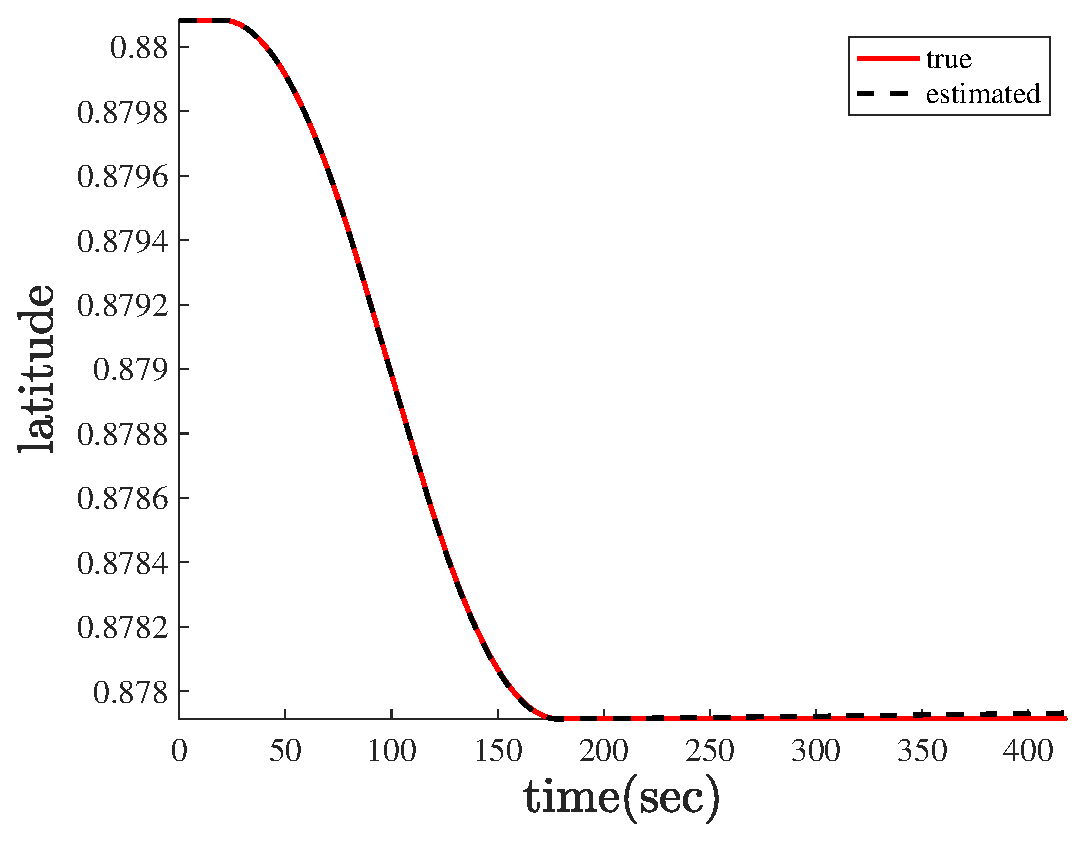
\includegraphics[width=0.7\textwidth]{../Figure/Q5/latitude_cos}
        \caption{Latitude}
    \end{figure}
    \begin{figure}[H]
        \centering
        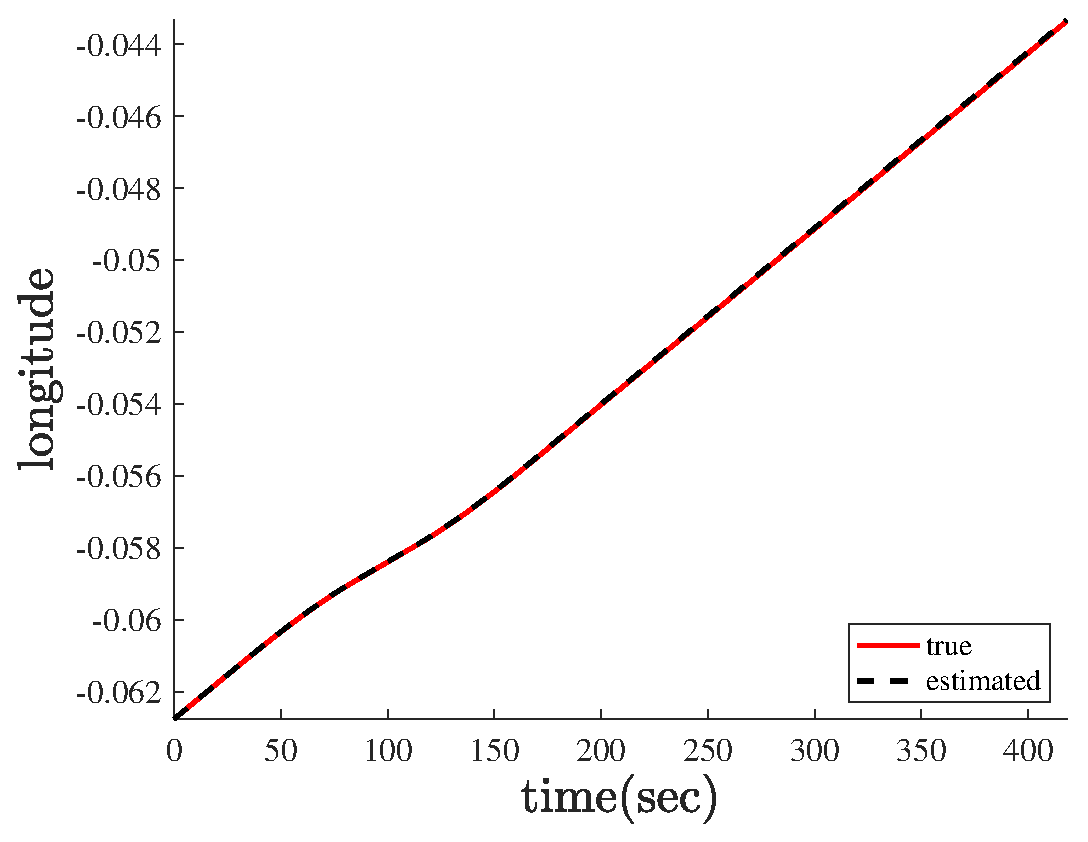
\includegraphics[width=0.7\textwidth]{../Figure/Q5/longitude_cos}
        \caption{Longitude}
    \end{figure}
    \begin{figure}[H]
        \centering
        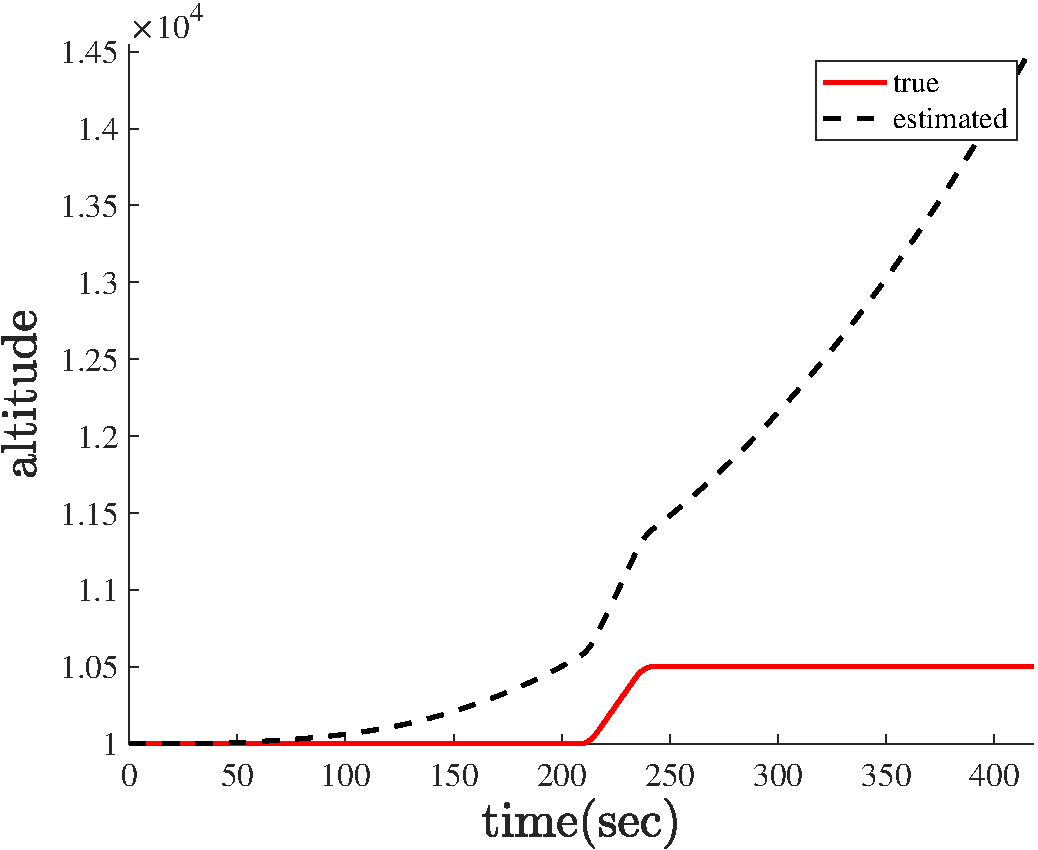
\includegraphics[width=0.7\textwidth]{../Figure/Q5/altitude_cos}
        \caption{Altitude}
    \end{figure}
    \begin{figure}[H]
        \centering
        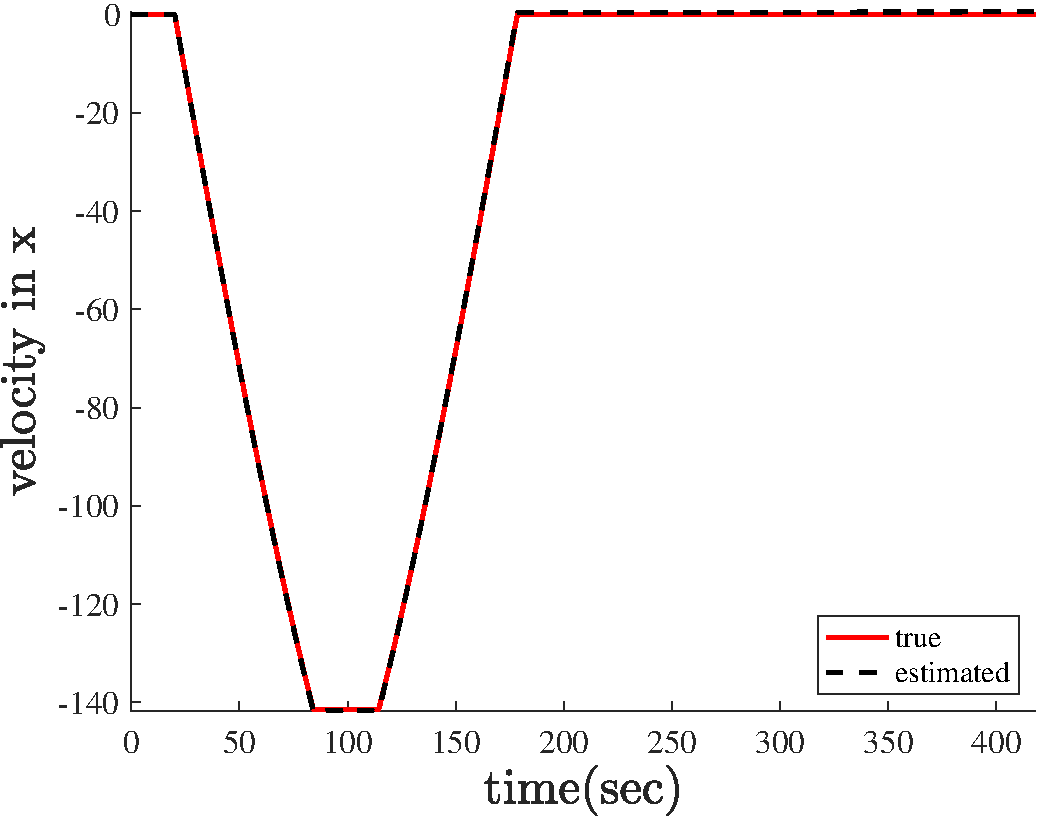
\includegraphics[width=0.7\textwidth]{../Figure/Q5/velocity_x_cos}
        \caption{Velocity in x direction}
    \end{figure}
    \begin{figure}[H]
        \centering
        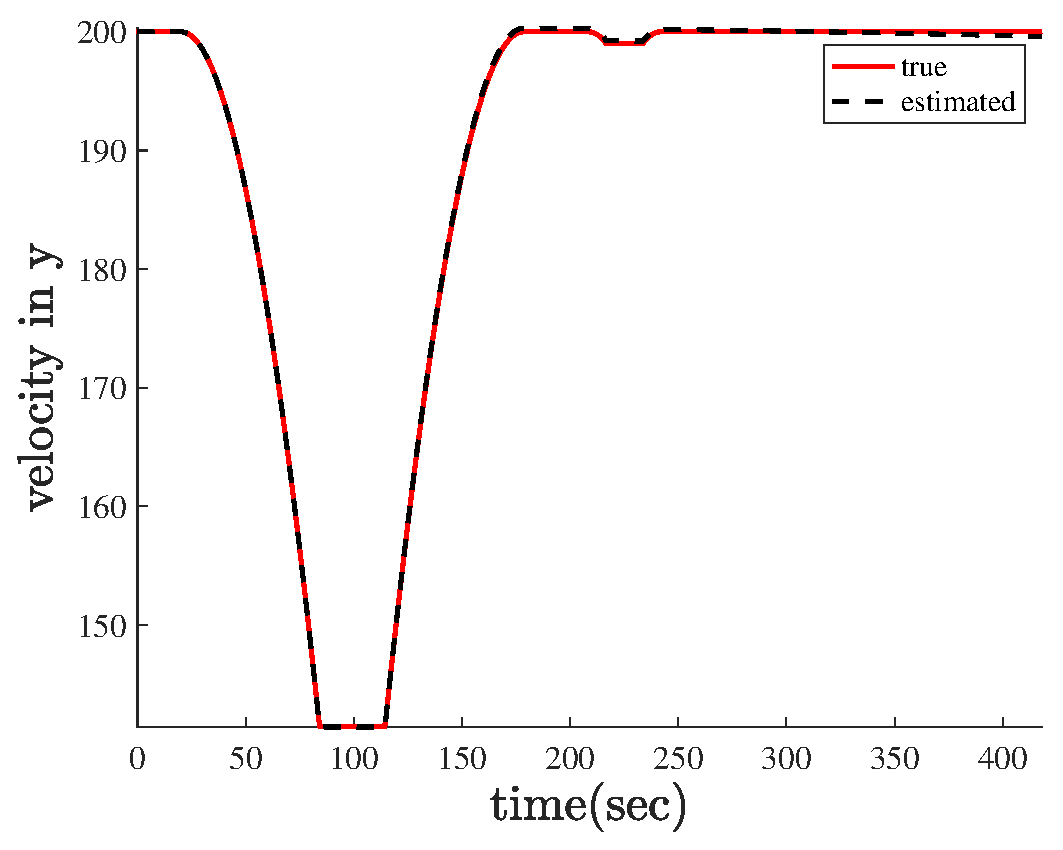
\includegraphics[width=0.7\textwidth]{../Figure/Q5/velocity_y_cos}
        \caption{Velocity in y direction}
    \end{figure}
    \begin{figure}[H]
        \centering
        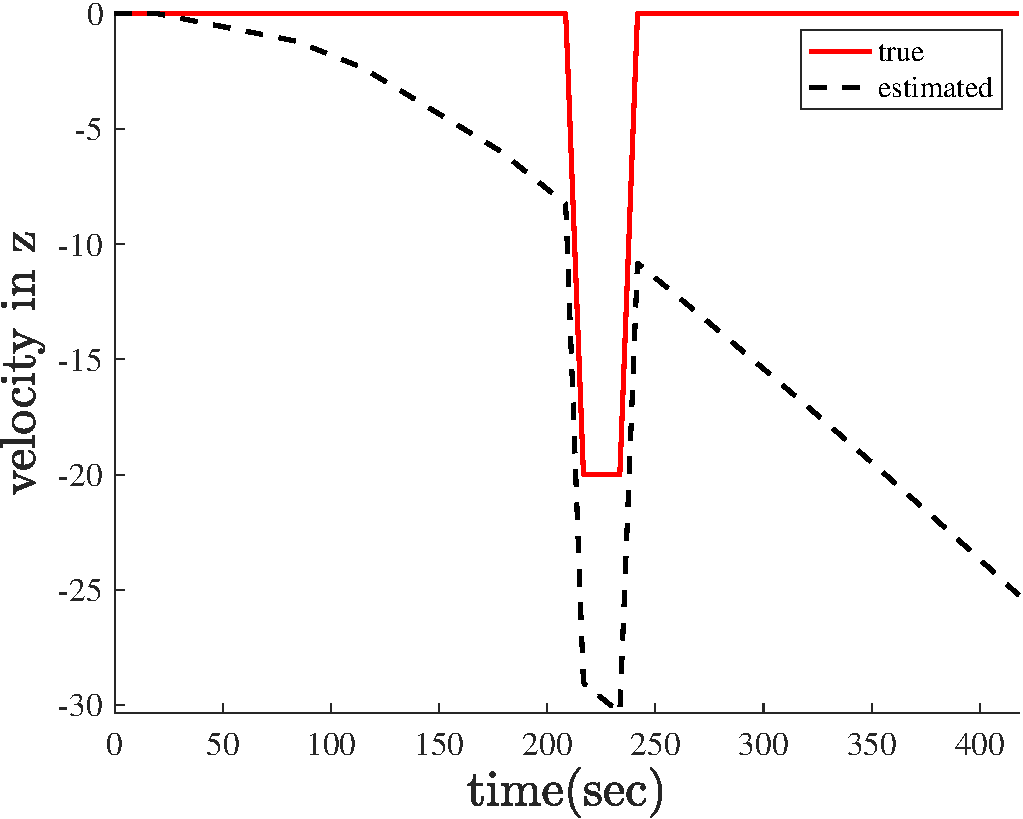
\includegraphics[width=0.7\textwidth]{../Figure/Q5/velocity_z_cos}
        \caption{Velocity in z direction}
    \end{figure}
    
    \begin{figure}
        \centering
        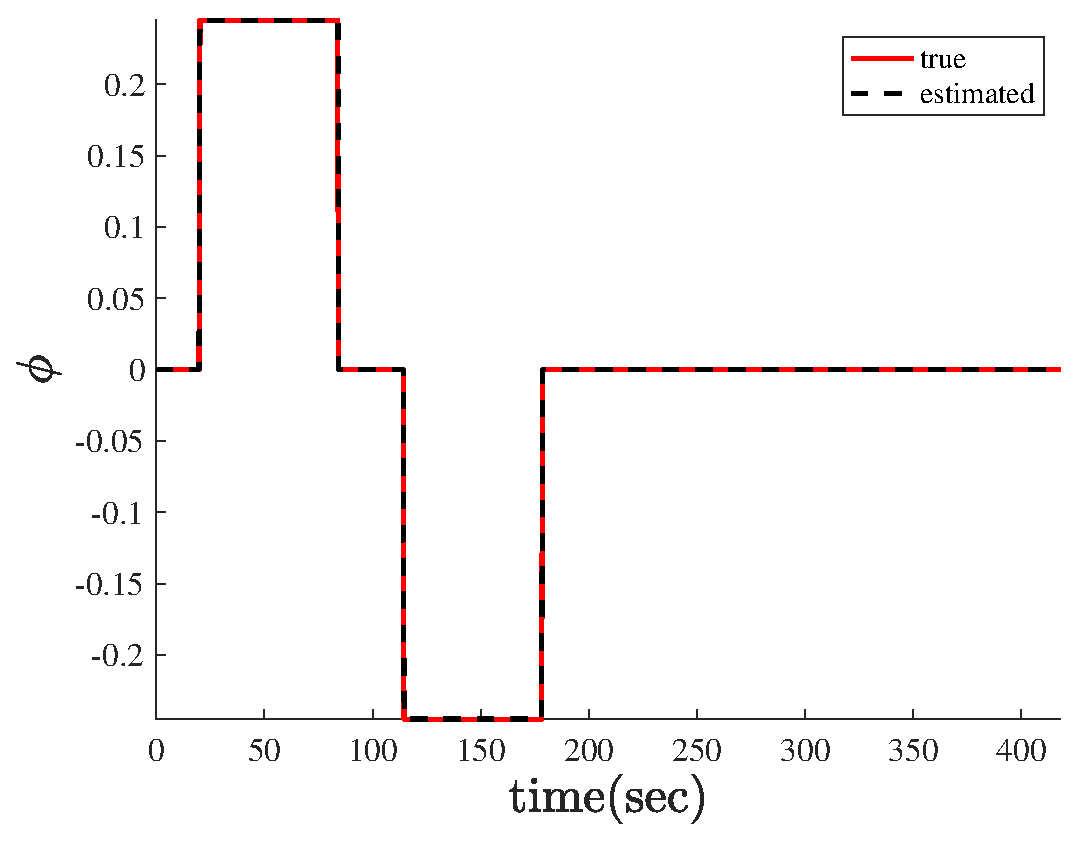
\includegraphics[width=0.7\textwidth]{../Figure/Q5/phi_cos}
        \caption{Roll}
    \end{figure}
    \begin{figure}
        \centering
        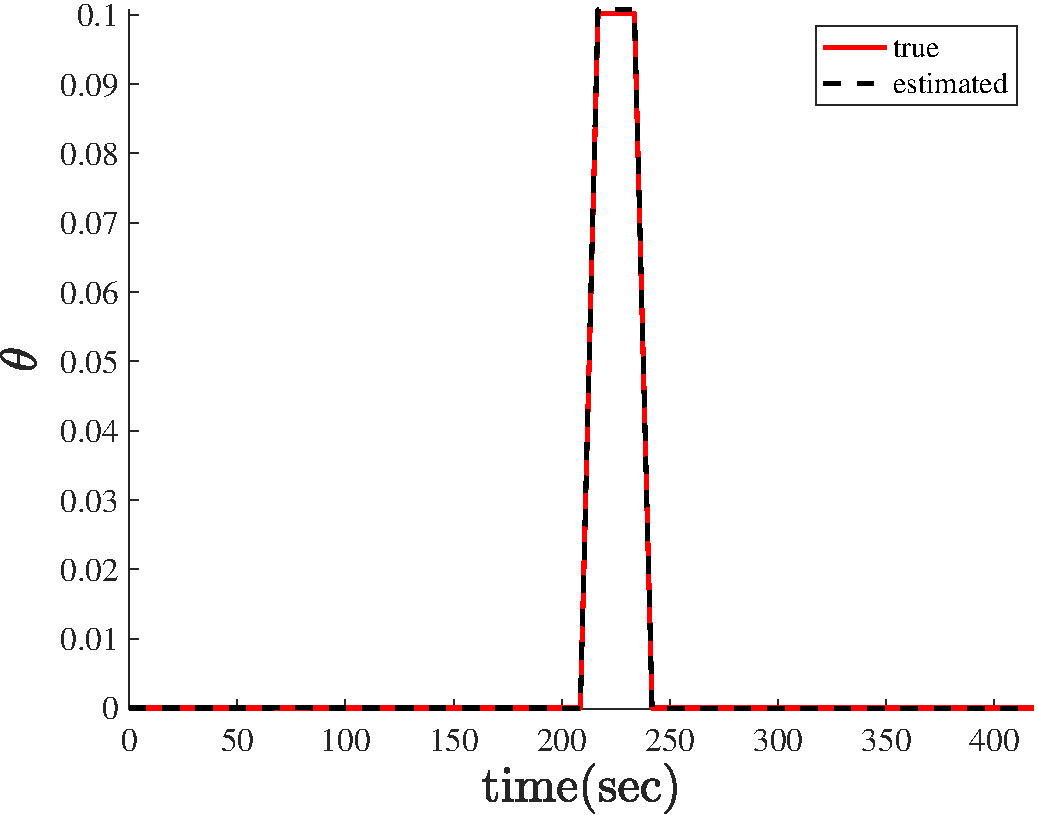
\includegraphics[width=0.7\textwidth]{../Figure/Q5/theta_cos}
        \caption{Pitch}
    \end{figure}
    \begin{figure}
        \centering
        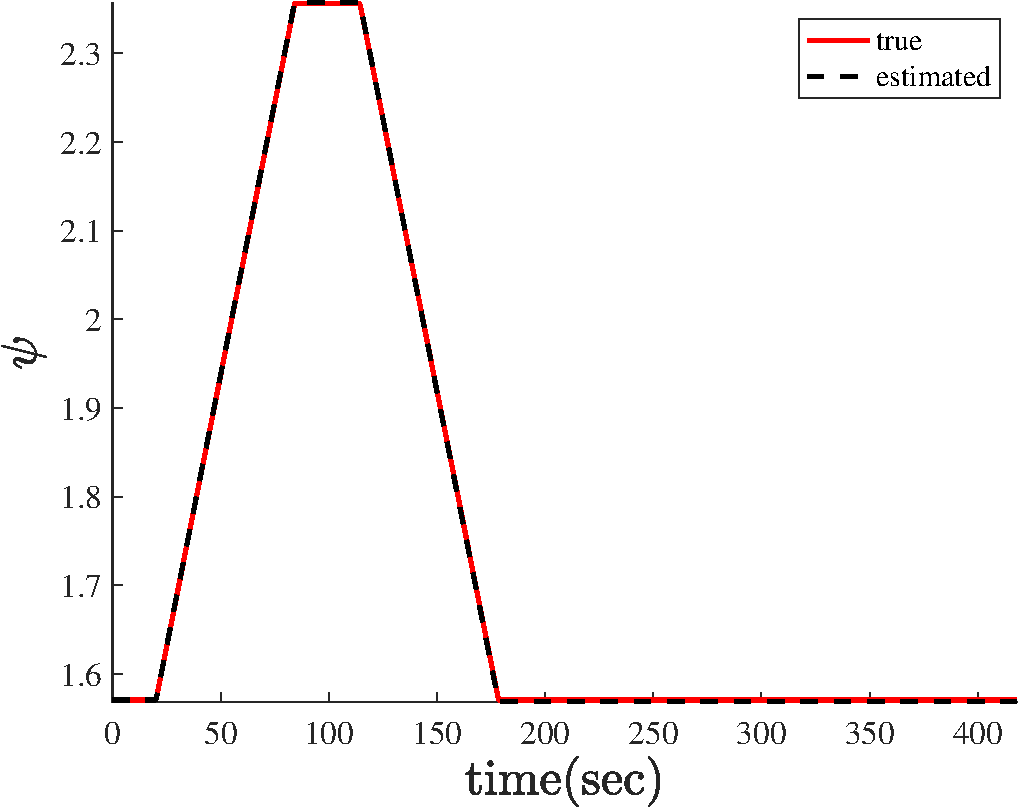
\includegraphics[width=0.7\textwidth]{../Figure/Q5/psi_cos}
        \caption{Yaw}
    \end{figure}






% \begin{align*}
% &\begin{bmatrix}
%     \cos(\phi)\tan(\theta)\sigma_6 - \sin(\phi)\tan(\theta)\sigma_8 & \cos(\psi)\sin(\theta)\sigma_{23} - \cos(\theta)\sigma_{28} \\
%     & -\cos(\phi)\tan(\theta)\sigma_{12} + \cos(\phi)\sigma_2\sigma_5 \\
%     & + \sin(\phi)\sigma_2\sigma_6 - \sin(\phi)\tan(\theta)\sigma_{11} - \frac{v_n\sin(\psi)\sin(\theta)}{R_m + h} \\
%     & \cos(\theta)\sin(\psi)\sigma_{23} - \cos(\phi)\tan(\theta)\sigma_{13} \\
%     & + \sin(\phi)\tan(\theta)\sigma_{14} + \frac{v_n\cos(\psi)\cos(\theta)}{R_m + h} \\
%     & \frac{\cos(\theta)\sin(\psi)}{R_m + h} - \frac{\cos(\phi)\tan(\theta)\sigma_{29}}{R_m + h} \\
%     & + \frac{\sin(\phi)\tan(\theta)\sigma_{27}}{R_m + h} \\
%     & \sin(\phi)\tan(\theta)\sigma_{17} - \cos(\phi)\tan(\theta)\sigma_{18} \\
%     & -\frac{\tan(L)\sin(\theta)}{R_m + h} - \frac{\cos(\psi)\cos(\theta)}{R_p + h} \\
%     & \cos(\phi)\tan(\theta)\sigma_{15} - \sin(\theta)\sigma_{24} \\
%     & + \cos(\phi)\tan(\theta)\sigma_{16} + \Omega_e\sin(L)\cos(\psi)\cos(\theta) \\
%     & 0 \\
%     & \sin(\phi)\tan(\theta)\sigma_{10} - \sin(\phi)\tan(\theta)\sigma_9 \\
%     & -\frac{v_n\cos(\theta)\sin(\psi)}{(R_m + h)^2} \\
%     & + \frac{v_e\tan(L)\sin(\theta)}{(R_m + h)^2} \\
%     & + \frac{v_e\cos(\psi)\cos(\theta)}{(R_p + h)^2}
% \end{bmatrix}
% \\
% &\begin{bmatrix}
%     \cos(\phi)\tan(\theta)\sigma_7 - \sin(\phi)\tan(\theta)\sigma_5 & 0 & \sin(\phi)\tan(\theta)\sigma_{15} \\
%     & \cos(\phi)\tan(\theta)\sigma_{16} + \Omega_e\sin(L)\cos(\psi)\cos(\theta) & 0 \\
%     \sin(\phi)\sigma_7 - \cos(\phi)\sigma_8 & \sin(\phi)\sigma_{12} - \cos(\phi)\sigma_{11} & 0 \\
%     \frac{\cos(\phi)\sigma_6}{\cos(\theta)} - \frac{\sin(\phi)\sigma_8}{\cos(\theta)} & \frac{\cos(\phi)\sin(\theta)\sigma_5}{\cos(\theta)^2} - \frac{\sin(\phi)\sigma_{11}}{\cos(\theta)} \\
%     & -\frac{\cos(\phi)\sigma_{12}}{\cos(\theta)} + \frac{\sin(\phi)\sin(\theta)\sigma_6}{\cos(\theta)^2} & 0 \\
%     \frac{\sin(\phi)\sigma_{27}}{\sigma_3} - \frac{\cos(\phi)\sigma_{29}}{\sigma_3} & \frac{\sin(\phi)\sigma_{17}}{\cos(\theta)} - \frac{\cos(\phi)\sigma_{18}}{\cos(\theta)} \\
%     & 0 & \frac{\cos(\phi)\sigma_{16}}{\cos(\theta)} + \frac{\sin(\phi)\sigma_{15}}{\cos(\theta)} \\
%     a_y\sigma_{26} + a_z\sigma_{25} & a_z\cos(\phi)\cos(\psi)\cos(\theta) - a_x\cos(\psi)\sin(\theta) \\
%     & a_y\cos(\psi)\cos(\theta)\sin(\phi) + a_z\sigma_{29} - a_y\sigma_{27} - a_x\cos(\theta)\sin(\psi) \\
%     & \frac{v_d}{R_m + h} \\
%     & -\sigma_4 - \frac{2v_e\tan(L)}{R_m + h} \\
%     -a_y\sigma_{29} - a_z\sigma_{27} & a_z\cos(\phi)\cos(\theta)\sin(\psi) - a_x\sin(\psi)\sin(\theta) \\
%     & a_y\cos(\theta)\sin(\phi)\sin(\psi) + a_z\sigma_{26} - a_y\sigma_{25} + a_x\cos(\psi)\cos(\theta) \\
%     & \sigma_4 + \sigma_{31} \\
%     & \frac{v_d}{R_p + h} + \frac{v_n\tan(L)}{R_m + h} \\
%     & \frac{v_e}{R_p + h} + \sigma_1 \\
%     & v_n(\sigma_1 + \sigma_{30}) - 2\Omega_ev_d\sin(L) \\
%     & -\frac{v_dv_e}{(R_p + h)^2} - \frac{v_ev_n\tan(L)}{(R_m + h)^2}
% \end{bmatrix}
% \end{align*}

